%Time-stamp: <2013-06-19 13:04:27 amoebe>
\documentclass{article}
\usepackage{natbib}
%\usepackage{fullpage}
\usepackage{graphics}
\usepackage{amsmath}
\usepackage{amssymb}
\usepackage[utf8]{inputenc}
\usepackage{longtable} % For splitting tables over pages
\usepackage{Sweave}
\usepackage{subfig}
\usepackage{fancyhdr}
\usepackage{lastpage}
\usepackage{timestamp}
%\usepackage[section] {placeins} % http://www.douglasvanbossuyt.com/2008/11/18/la%\SweaveOpts{keep.source=TRUE} % don't remove source code comments
 % save auto-generated figures in
                                % figs/, prefixed by cant-f0creak-

\setlength{\bibsep}{0.0pt}
\setlength{\headheight}{15.2pt}
\setlength{\headsep}{12pt}
\pagestyle{fancyplain}
\fancyhf{}

\lhead{Kristine M. Yu}
\rhead{ldc-kiy plots for Example 2.3.3 in paper from 20111213, \timestamp}
\cfoot{\thepage\ of \pageref{LastPage}}

\begin{document}

I added prefixes of T to the tone labels in the hash table using the following:

\begin{verbatim}
awk -F '\t' -v OFS='\t' '{$4="T"$4} {$5="T"$5} {print}' 20111213-1-kiy-ap-framedwordlist.txt > 20111213-1-kiy-ap-framedwordlist-new.txt 
\end{verbatim}


\begin{figure}[h]
  \centering

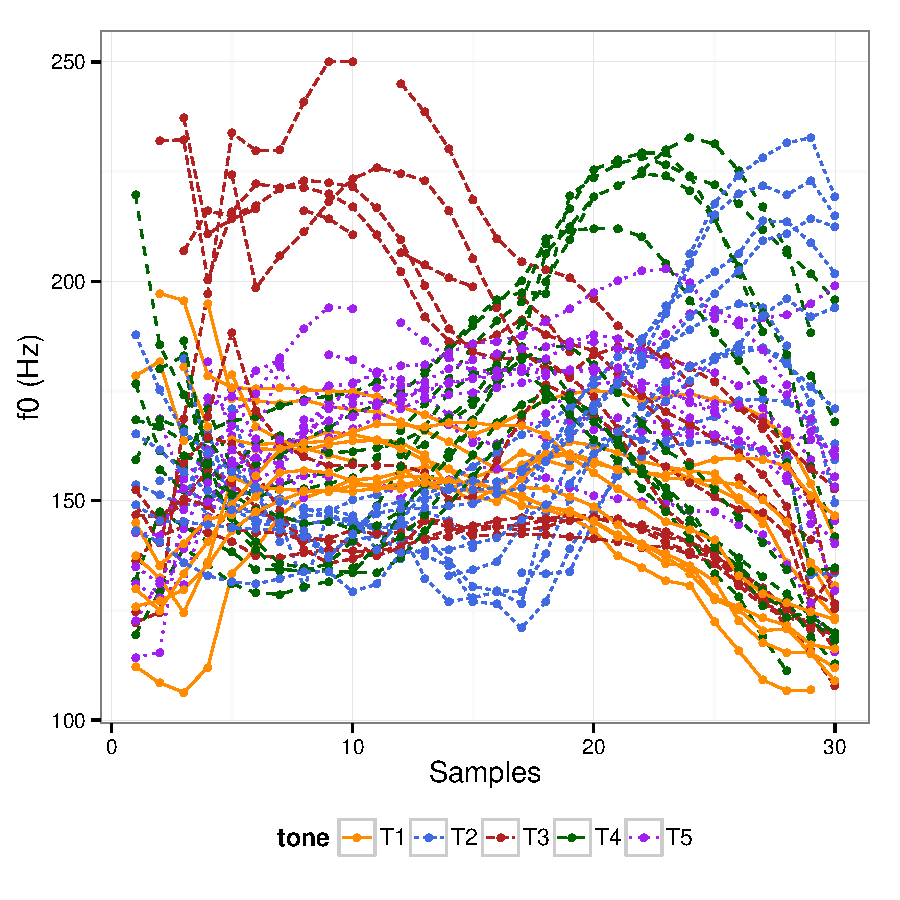
\includegraphics{figs/kiy-20111213-plot-all-by-tone}

\caption{All tones on top of one another.}
  \label{fig:plot-all-by-tone}
\end{figure}

\clearpage


\begin{figure}[h]
  \centering

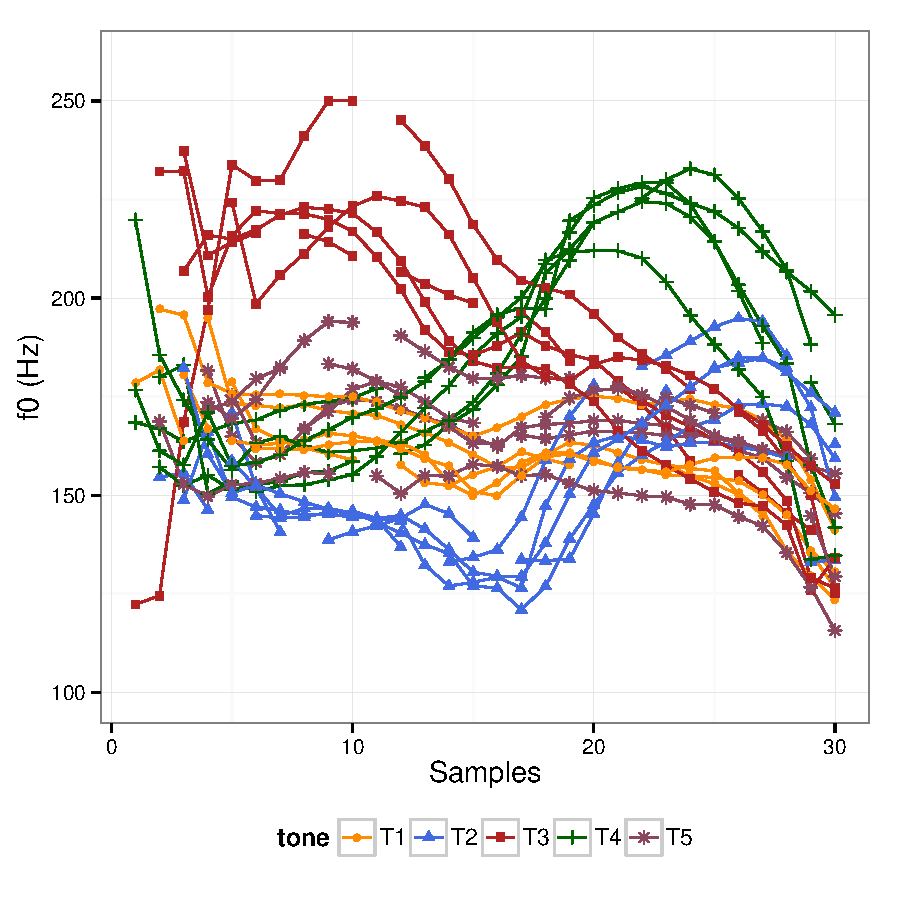
\includegraphics{figs/kiy-20111213-plot-w1}

\caption{All tones for word 1}
  \label{fig:plot-w1}
\end{figure}

\clearpage


\begin{figure}[h]
  \centering

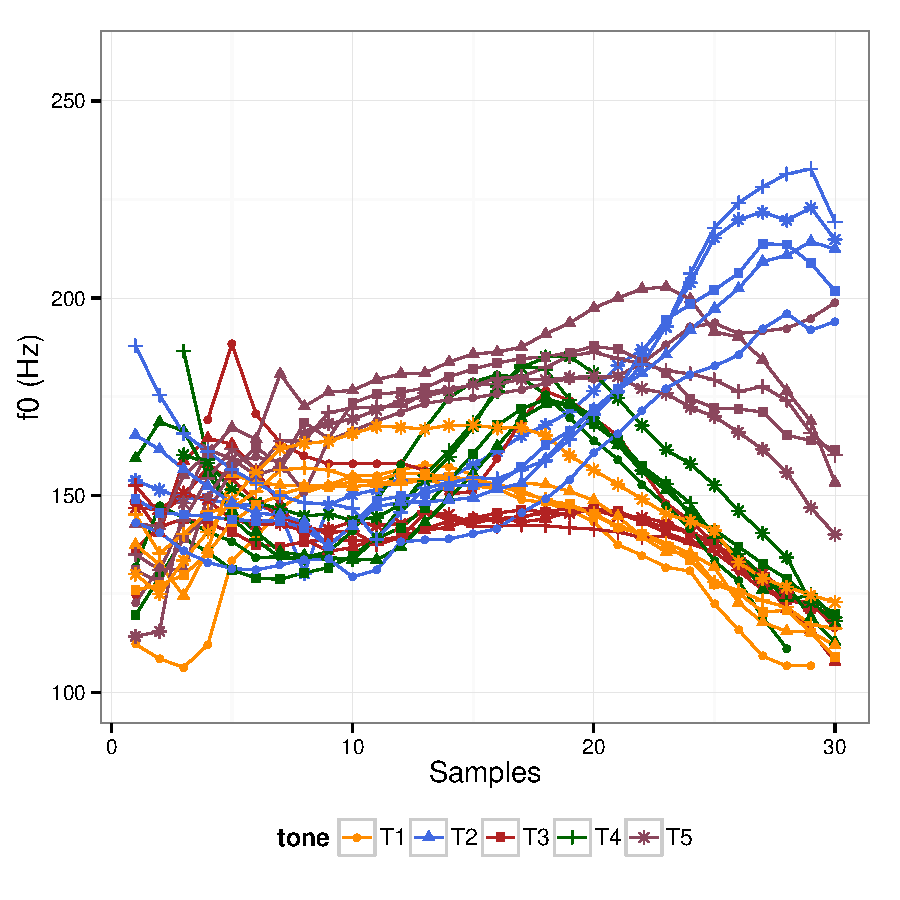
\includegraphics{figs/kiy-20111213-plot-w2}

\caption{All tones for word 2}
  \label{fig:plot-w2}
\end{figure}

\clearpage


\begin{figure}
  \centering

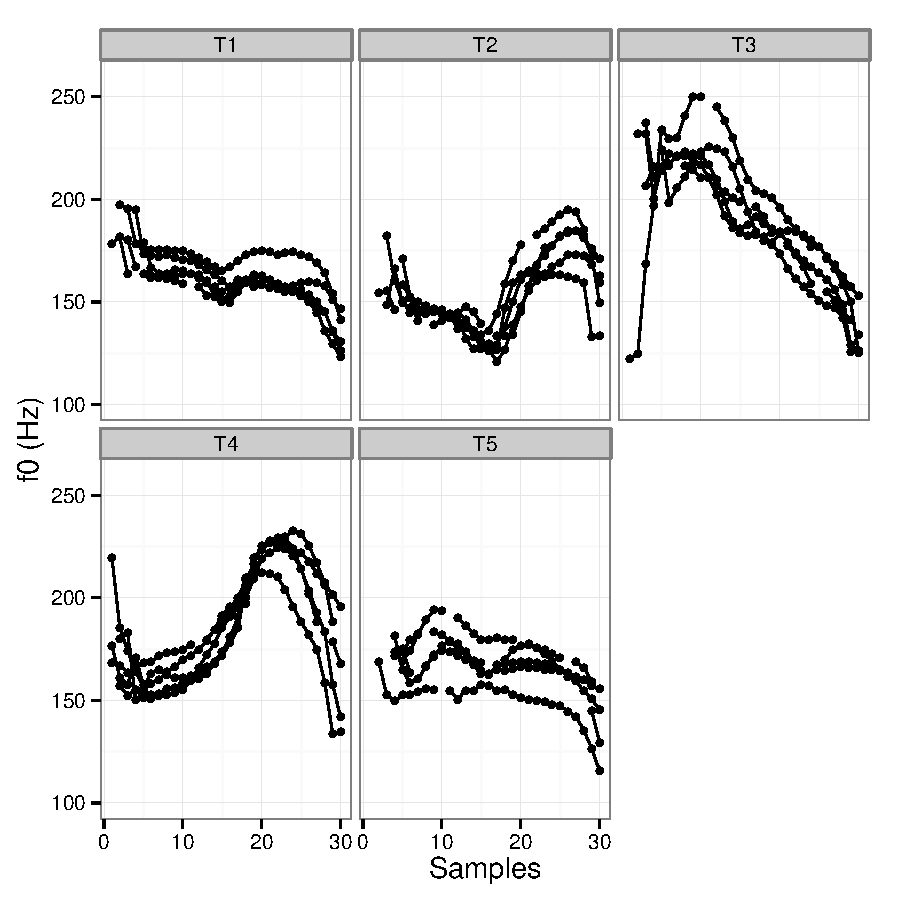
\includegraphics{figs/kiy-20111213-plot-w1-facet}

\caption{All tones for word 1, faceted}
  \label{fig:plot-w1}
\end{figure}

\clearpage


\begin{figure}
  \centering
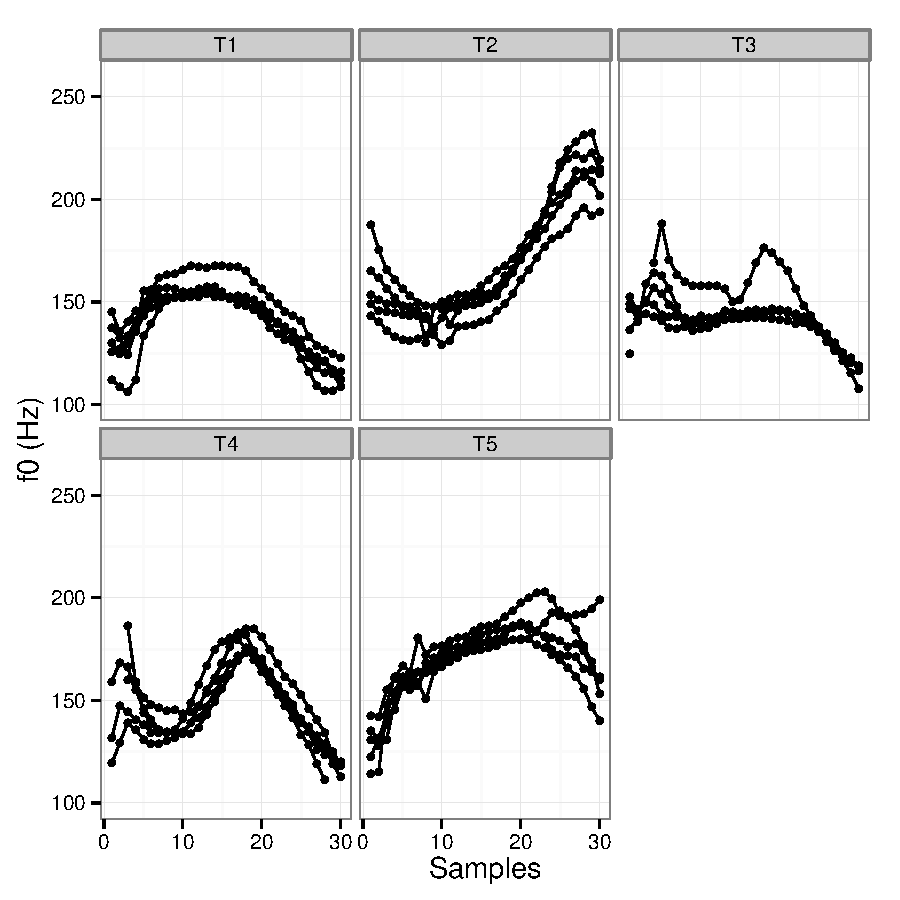
\includegraphics{figs/kiy-20111213-plot-w2-facet}

\caption{All tones for word 2, faceted}
  \label{fig:plot-w2-facet}
\end{figure}

\clearpage

\end{document}

